\chapter{Das Referenzmodell: Einzelne Kugel auf festem Grund}



\section{Erstellung und Equilibrierung der Probe}
	Eine Probe im Sinne der MD ist eine Datei, welche mindestens alle notwendigen Eigenschaften
	aller Teilchen im System speichert. Dazu gehören natürlich der Ort und die Geschwindigkeit
	jedes Teilchens, aber auch der Teilchentyp und die Teilchenmasse. Der Mulde im LJ-Potential
	\eqref{eq:potential_lj} nach gibt es für alle Teilchen einen Zustand minimaler Energie.
	Aus diesem Grund existiert ein stationärer Gleichgewichtzustand (\emph{Equilibrium}). Den
	Gesetzen der Thermodynamik nach geht jedes ungestörte Nichtgleichgewichtssystem in sein
	Equilibrium über. Dieser Vorgang heißt \emph{Equilibrierung}. Da eine digital für eine
	Simulation erstellte Probe prinzipiell einen beliebigen Zustand haben kann, ist eine
	\emph{vorherige} Equilibrierung besonders wichtig. Andernfalls findet der
	Equilibrierungsprozess während der eigentlichen Simulation statt, was zu verfälschten
	Ergebnissen führen kann.

	Für das Modell dieser Arbeit bietet es sich an, eine auf \SI{300}{\kelvin} aufgeheizte Probe
	zu betrachten. Viele der in der Literatur auffindbaren Vergleichswerte zu Materialkonstanten
	werden bei diesem der Raumtemperatur nahe gelegenen Wert angegeben. Zudem bildet es das
	Problem gut ab.

	\subsection{Homogene Deformation}
		Um eine Probe nun in ihren Gleichgewichtszustand bei dieser Temperatur zu versetzen bietet
		es sich an, eine Probe der Temperatur \SI{0}{\kelvin} zu erstellen und diese nach ihrer
		Equilibrierung aufzuheizen. Dies lässt sich einfach dadurch erreichen, dass die
		Teilchengeschwindigkeiten auf 0 gesetzt werden. Mithilfer einer homogenen Deformation wird
		eine Simulation ohne Berücksichtigung der durch die Kraft verursachten Teilchenbewegungen
		durchgeführt. In jedem Simulationsschritt wird die Probe mithilfe einer zum Gitter
		achsenparallelen Deformationsmatrix skaliert. Die sich dadurch ergebende mittlere
		potentielle Energie kann un minimiert werden. Aufgrund der Proportionalität zwischen dem
		Druck $P$ und den gemittelten Kräften äußert sich diese Stelle in Abbildung
		\ref{fig:homdef} in Form einer Nullstelle. Dies ist auch in sofern einleuchtend, da der
		Druck angibt, inwiefern sich einen Probe zusammenziehen oder ausdehnen würde.

		\begin{figure}[!ht]
			\centering
			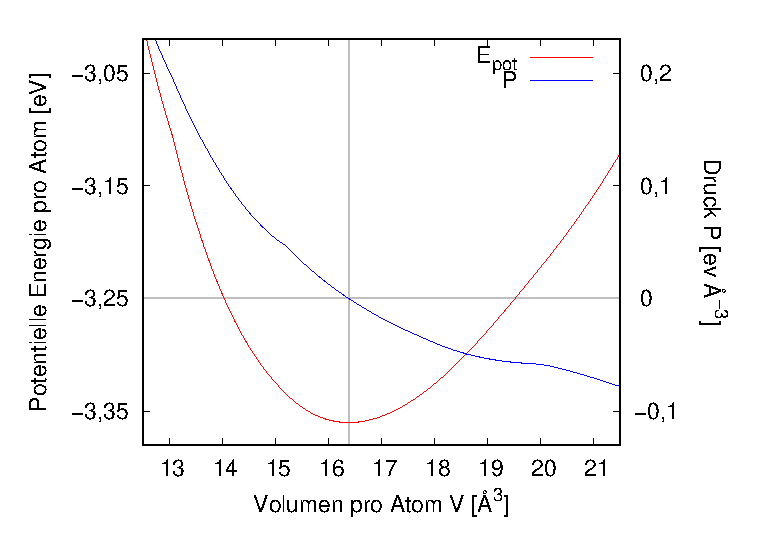
\includegraphics[width=0.9\textwidth]{chapter/main/single/plt/equilibration/homdef.eps}
			\caption{Die mittlere potentielle Energie und der Probendruck aufgetragen gegen das
			Volumen pro Teilchen. Das Energieminimum kann durch einen näherungsweise quadratischen
			Fit um das Minimum oder über den Nulldurchlauf des Druckverlaufs bestimmt werden. In
			diesem Fall liegt das Energieminimum bei einem Teilchenvolumen von
			\SI{16.38}{\angstrom\cubed}.}
			\label{fig:homdef}
		\end{figure}

	\subsection{Aufheizen der Probe}
		Die bisherige Simulation fand unter Beachtung der Regeln eines mikrokanonischen Ensembles
		(\emph{NVE}) statt. Das bedeutet, dass neben der Teilchenzahl $N$ und dem Volumen $V$ die
		Gesamtenergie $E$ festgehalten wurde. Da im nächsten Schritt eine Energiezufuhr zum
		Aufheizen der Probe notwendig ist, ist dieses System so nciht zwangsläufig geeignet.
		Stattdessen bietet sich das kanonische Ensemble (\emph{NVT}) an. Hier werden auch die
		Teilchenzahl und das Volumen fest gesetzt, allerdings wird hier statt der Energie die
		Temperatur $T$ durch Kopplung an ein Wärmebad vorgegeben. In der SImulation wird dies
		mithilfe eines Thermostats realisiert. Ein Theromostat maipuliert dabei die Simulation in
		der Hinsicht, dass die Temperatur der vorgabe entspricht. Ein einfacher Thermastat wäre
		das Berendsen-Thermostat, bei dem der durch das Äquipartitionstheorem
		\eqref{eq:equipartition} gegegbene Zusammenhang zwischen Temperatur und
		Teilchengeschwindigkeit genutzt wird, um alle Teilchengeschwindigkeiten global zu
		reskalieren. Dies hat allerdings einen Verlust der Poisson-Verteiltheit der
		Geschwindigkeiten zur Folge. Der in IMD verwendete Thermostat ist deshalb das
		\emph{Nosé-Hoover-Thermostat} \cite{rapp2014laserablation}.

		\begin{figure}[!ht]
			\centering
			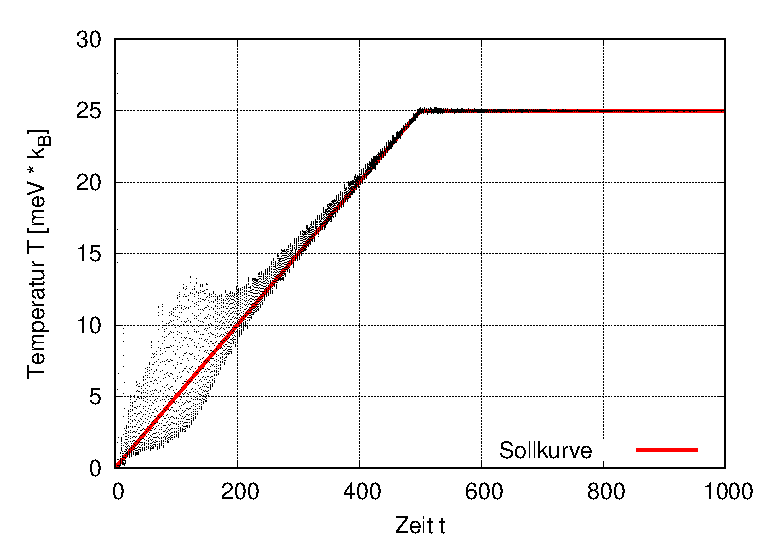
\includegraphics[width=0.9\textwidth]{chapter/main/single/plt/equilibration/thermostat.eps}
			\caption{Der Aufheizprozess mit vorgegebener Temperatur. Die Fluktuationen werden
			mit fortschreitender Zeit geringer.}
			\label{fig:thermostat}
		\end{figure}

		Abbildung \ref{fig:thermostat} zeigt das Aufheizen einer würfelförmigen Probe mithilfe des
		in IMD implementierten Nosé-Hoover-Thermostats. Während die Temperatur am Anfang trotz
		Vorgabe noch schwankt, vermindert sich dieser Effekt mit der Zeit. Ab ungefähr 800
		Zeiteinheiten sind die Fluktuationen in etwas konstant.

		\begin{figure}[!ht]
			\centering
			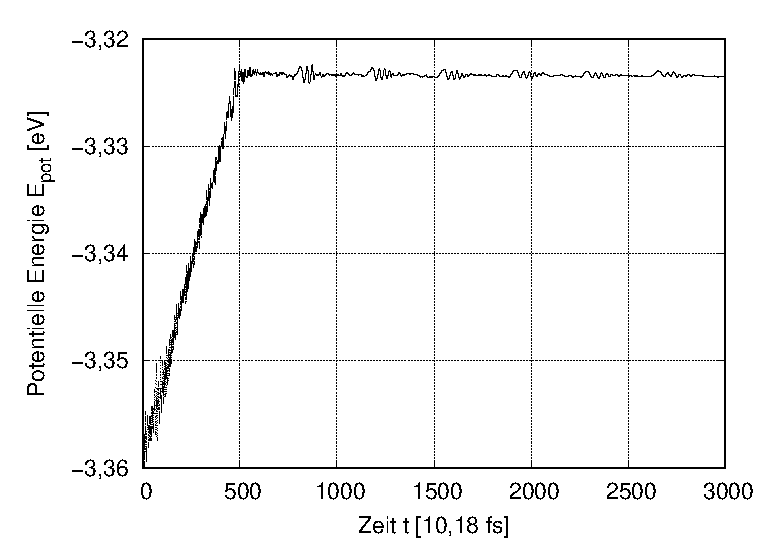
\includegraphics[width=0.9\textwidth]{chapter/main/single/plt/equilibration/thermostat_pot.eps}
			\caption{Die potentielle Energie zeigt einen zur Temperatur proportionalen Verlauf}
			\label{fig:thermostat_pot}
		\end{figure}

		Wie allerdings in Abbildung \ref{fig:thermostat_pot} zu sehen ist, verhält sich die
		potentielle Energie proportional zum Temperaturverlauf. Von daher ist es ratsam nach dem
		Aufheizen eine NVE-Simulation bis zum Equilibrium durchzuführen.

	\subsection{Zuschneiden der Probe}
		Üblicherweise sind Proben quaderförmig. Im Rahmen dieser Arbeit sind jedoch Kugelformen
		unter der Einwirkung von Gravitation interessant, da sie so den Pulverpartikeln beim
		SLM-Verfahren am ähnlichsten sind. Die einfachste Methode zum erzeugen einer solchen Probe
		ist das Entfernen der entsprechenden Teilchen aus einem Quader. Aus diesem Grund stellt
		sich die Frage zu welchen Zeitpunkt das Zuschneiden am geschicktesten wäre.

		\begin{figure}[!ht]
			\centering
			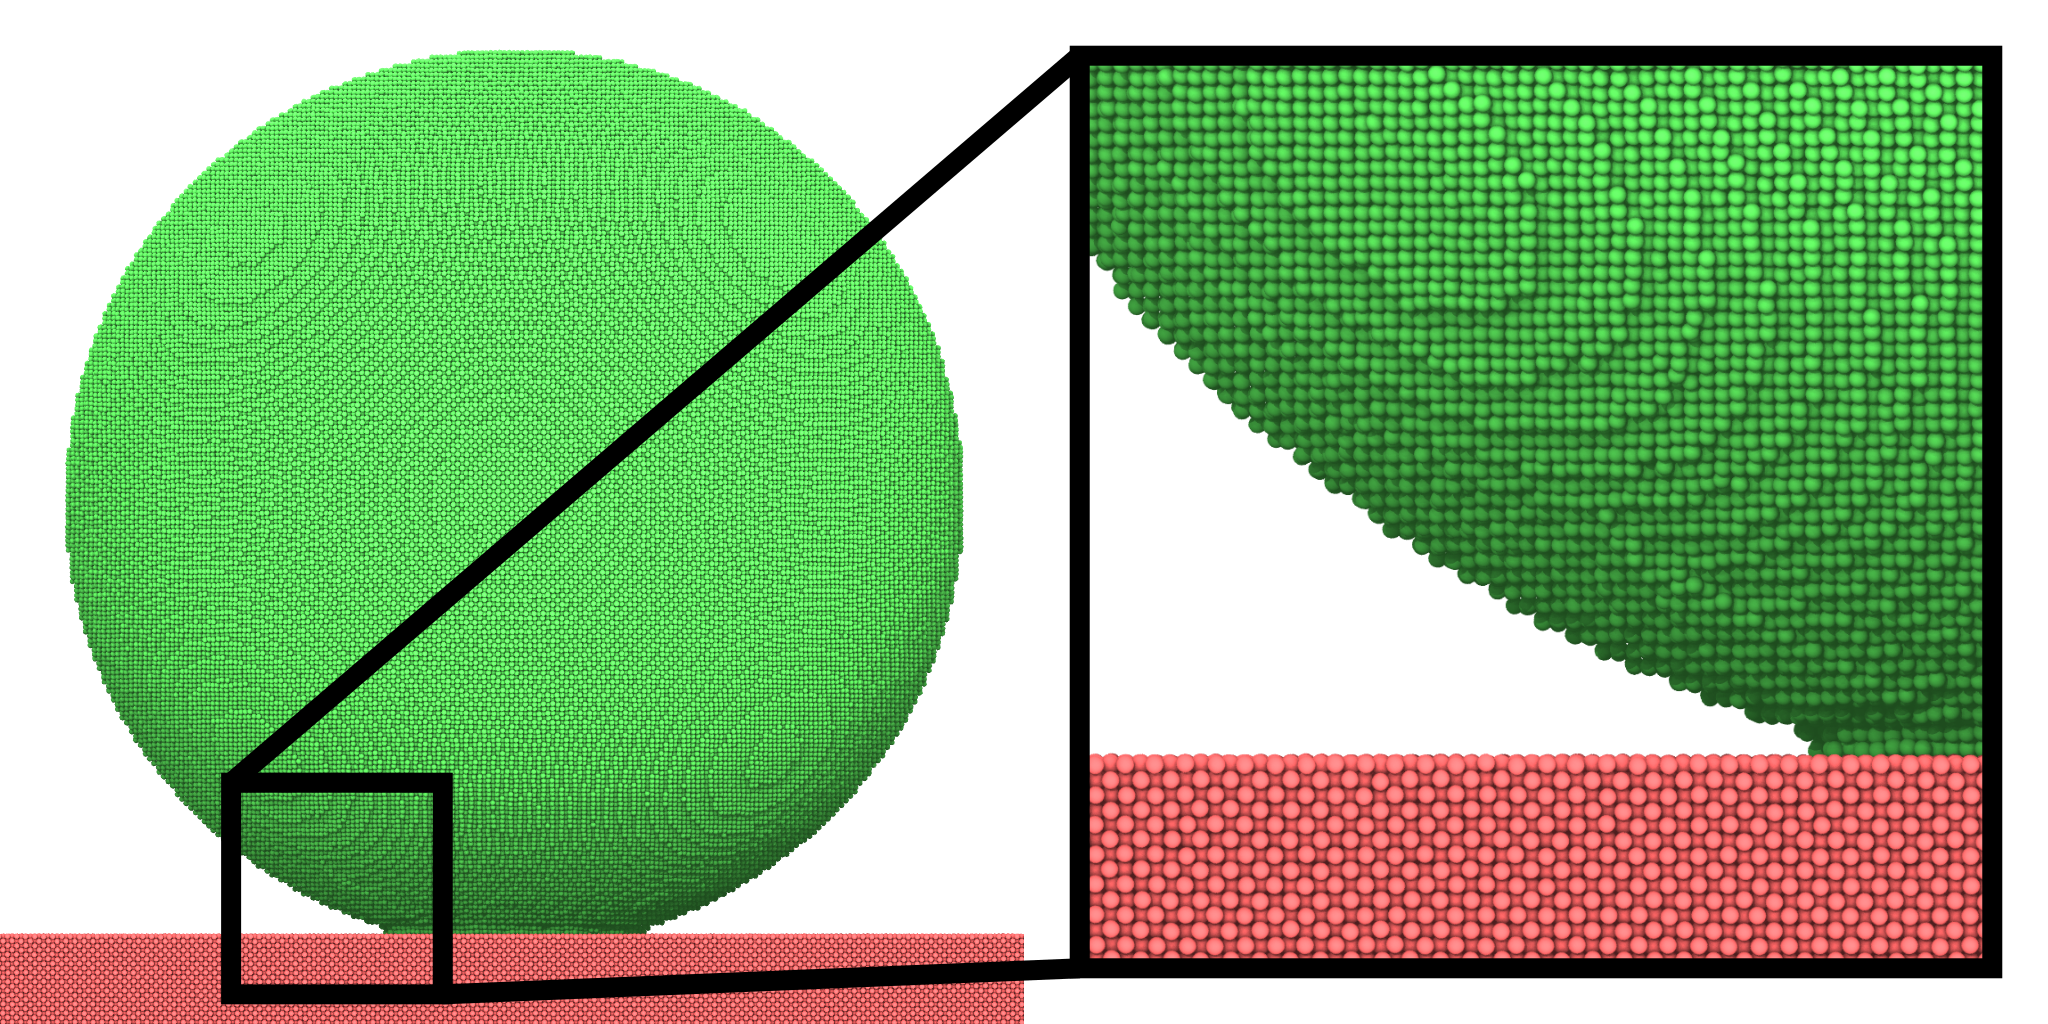
\includegraphics[width=\textwidth]{chapter/main/single/img/equilibrated_sphere.zoom.png}
			\caption{Eine vollständig equilibrierte Kugel aus Aluminiumatomen auf einem festen,
			unbeweglichen Untergrund}
			\label{fig:equilibrated_sample}
		\end{figure}

		Tatsächlich hat sich gezeigt, dass es am geschicktesten ist, die Kugel vor dem Aufheizen,
		aber nach der homogenen Deformation freizustellen. So behält die homogene Deformation ihr
		Gültigkeit, das freigestellte Material kann aber an seinen neuen Rändern relaxieren, ohne
		dass später sowieso entfernte Teilchen Einfluss auf das Verhalten an der Oberfläche
		nehmen. Diese kann (vor allem unter Gravitation) eine vom kugelförmigen Gitterausschnitt
		leicht verschiedene Oberflächenform annehmen annehmen, die im Gitter mit periodischen
		Randbedingungen gar nicht zustandekommen könnte. Ein Freischneiden nach der vollständigen
		Equilibrierung hätte zu einem Absacken der Kugel während der eigentlichen Simulation
		geführt, sodass dies das Ergebnissen hätte beeinflussen können.


\section{Kalibrierung der Laserleistung bei fester Lasergeschwindigkeit}
\todo[color=green]{Vielleicht geschmolzenenen Anteil gehen? Eventuell Kapitelaufteilung in verschiedene Leistungen?}

\section{Verhalten bei halbierter Lasergeschwindigkeit}
